\subsection{Klassifikation der endlichen orthogonalen Gruppen}
Nachdem wir uns mit den orthogonalen Abbildungen im zweidimensionalen Raum vertraut gemacht und ihre besonderen Eigenschaften kennengelernt haben, möchten wir uns mit der Klassifizierung von endlichen Untergruppen der orthogonalen Gruppe befassen.

Der nachfolgende Satz \ref{klassO(R2)} teilt die endlichen Untergruppen der orthogonalen Gruppe in zwei Klassen ein, einmal in die Untergruppen vom Typ der zyklischen Gruppe und in die vom Typ der Diedergruppe.
\begin{theorem}\label{klassO(R2)}
	Sei $\mathcal{G}$ eine endliche Untergruppe von $\OR{2}$, dann ist $\mathcal{G}$ entweder eine zyklische Gruppe $\mathcal{C}^n_2$ oder eine Diedergruppe $\mathcal{H}^n_2$ für $n \in \mathbb{N}$.
\end{theorem}
Bevor wir diesen Satz beweisen, sollten wir uns vorher die Definitionen der Diedergruppe, der zyklischen Gruppe und der Nebenklassen anschauen und nachvollziehen.
\begin{defi}[Zyklische Gruppe]
	Eine Gruppe $\mathcal{C}$ heißt zyklisch, wenn sie ein Element $A$ enthält, sodass für jedes Element $B$ von $\mathcal{C}$ ein $n \in \mathbb{Z}$ existiert, sodass $A^n = B$. Außerdem gilt, dass $\mathcal{C}$ die einzige Untergruppe von $\mathcal{C}$ ist, die $A$ enthält. Dann nennen wir $A$ den Erzeuger von $\mathcal{C}$ und können schreiben $\mathcal{C} = \langle A \rangle$.
\end{defi}
Damit wir die Definition der zyklischen Gruppe besser verstehen können, werden wir uns eine Gruppe anschauen und überprüfen, ob diese zyklisch ist.

Wir wählen dazu die Gruppe $\mathcal{C}_4$ aus. Diese Gruppe enthält alle möglichen Drehungen der Ebene, die ein Quadrat in sich überführen. Also besteht die Gruppe (wie in Abbildung \ref{fig:zyklische_gruppe_c4} zu erkennen ist) aus den Drehungen um $90^{\circ}$, $180^{\circ}$, $270^{\circ}$ und $0^{\circ}$, da Drehwinkel immer modulo $360^{\circ}$ gerechnet werden.
\begin{figure}[H]
	\centering
	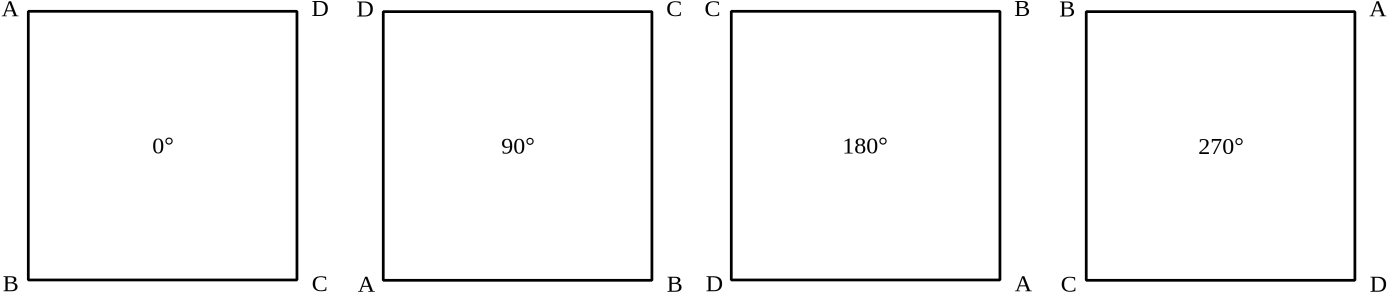
\includegraphics[width=1\linewidth]{grafiken/zyklische_gruppe_c4}
	\caption{Grafische Darstellung der Elemente von $\mathcal{C}_4$}
	\label{fig:zyklische_gruppe_c4}
\end{figure}
Um zu überprüfen, ob diese Gruppe zyklisch ist, können wir nun versuchen die Definition der zyklischen Gruppe anzuwenden. Zuerst wählen wir das Element $A$, die Drehung um $90^{\circ}$. Wir müssen nun zeigen, dass wir jedes andere Element der Gruppe mit dem Element $A$ darstellen können. Dies können wir natürlich. Damit wir die Drehung um $180^{\circ}$ darstellen können, müssen wir $A$ mit sich selbst verknüpfen. Um $270^{\circ}$ darzustellen müssen wir $A$ dreimal mit sich selbst verknüpfen. Da wir nun alle Element der Gruppe $\mathcal{C}_4$ mit $A$ darstellen können, haben wir herausgefunden, dass die Gruppe eine zyklische Gruppe mit Erzeuger $A$, der Drehung um $90^{\circ}$, ist. \par\smallskip
Wenn wir auch Spiegelungen zulassen, dann erhalten wir im Falle von regelmäßigen Polygonen eine Diedergruppe.
\begin{defi}[Diedergruppe]
	Eine Gruppe $\mathcal{H}$ ist eine Diedergruppe, wenn sie die Isometriegruppe eines regelmäßigen $n$-Ecks in der Ebene ist. Sie besteht dann aus $n$ Drehungen und $n$ Spiegelungen, also aus insgesamt $2n$ Elementen.
\end{defi}
Auch für Diedergruppen möchten wir uns ein Beispiel anschauen, dazu können wir uns aus vorherigen Beispiel bedienen und wie schon erwähnt noch Spiegelungen der Gruppe hinzufügen, die das Viereck in sich selber überführen.
\begin{figure}[H]
	\centering
	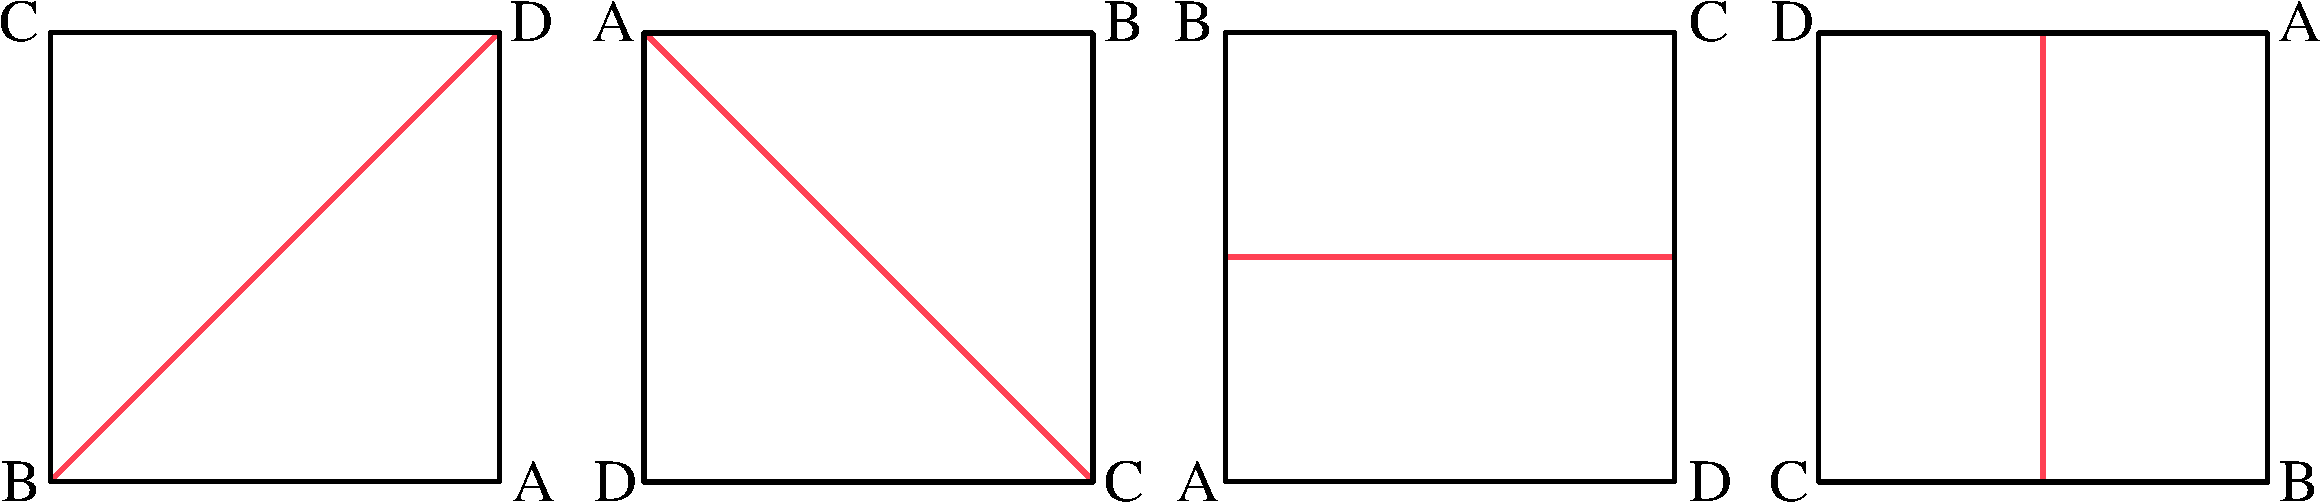
\includegraphics[width=1\linewidth]{grafiken/dieder_gruppe}
	\caption{Grafische Darstellung der Elemente von $\mathcal{D}_4$}
	\label{fig:zyklische_gruppe_d4}
\end{figure}
Wie in der Abbildung \ref{fig:zyklische_gruppe_d4} zu sehen ist, kommen auf diese Weise vier weitere Elemente zu der Gruppe hinzu. Diese vier Spiegelungen zusammen mit den vier Drehungen vom vorherigen Beispiel bilden die Diedergruppe $\mathcal{D}_4$. Diese Gruppe wird von zwei Elementen erzeugt, zum einen von dem Erzeuger der zyklischen Gruppe $\mathcal{C}_4$ und zum anderen von einer der vier Spiegelungen.
\begin{defi}[Linksnebenklasse]
	Zu einer Untergruppe $\mathcal{H} \subseteq \mathcal{G}$ heißt eine Teilmenge der Form $g\mathcal{H} = \{gh|h\in\mathcal{H}\}$ mit $g \in G$ eine Linksnebenklasse. Die Anzahl der Linksnebenklassen heißt der Index von $\mathcal{H}$ in $\mathcal{G}$.
\end{defi}
Als Beispiel nehmen wir uns die Diedergruppe $\mathcal{D}_4$, mit der wir uns schon vertraut gemacht haben. Die zyklische Gruppe $\mathcal{C}_4$ ist eine Untergruppe der Diedergruppe mit Index 2. Es ist leicht zu sehen, dass die zyklische Gruppe eine Untergruppe der Diedergruppe ist. Wir können die zyklische Gruppe auch als Linksnebenklasse auf"|fassen, indem wir die Gruppe von links mit Einheitsmatrizen verknüpfen. Eine zweite Linksnebenklasse, die wir finden können, entsteht durch die Verknüpfung einer beliebigen Spiegelung der Diedergruppe mit der zyklischen Gruppen. Wenn wir nun beide Linksnebenklassen miteinander vereinigen, erhalten wir die vollständige Diedergruppe. Daher hat die zyklische Gruppe in der Diedergruppe den Index 2. \par\smallskip
Da wir nun wichtige Definitionen für Satz \ref{klassO(R2)} wiederholt und anhand von Beispielen angewendet haben, können wir nun mit dem Beweis des Satzes beginnen.
\begin{proof}[Beweis von Satz 2.1]
	 Zunächst wollen wir zeigen, dass eine beliebig gewählte endliche Untergruppe von $\OR{2}$, die nur Drehungen enthält, eine zyklischen Gruppe sein muss. \par\smallskip
	 Sei $\mathcal{G}$ eine beliebige endliche Untergruppe von $\OR{2}$. Wir nehmen an, dass $\mathcal{H} \leq \mathcal{G}$ eine Untergruppe in $\mathcal{G}$ ist, die alle Drehungen in $\mathcal{G}$ enthält.

	 Wir wollen zeigen, dass $\mathcal{H}$ zyklisch sein muss. Für $|\mathcal{H}|=1$ ist dies bereits klar. Wenn $|\mathcal{H}| \neq 1$, wählen wir eine Drehung $R \in \mathcal{H}$, sodass $R \neq E_2$ und der Drehwinkel $\theta(R)$ minimal ist. Wenn wir jetzt eine weitere Drehung $T \in \mathcal{H}$ nehmen, dann können wir ein $m \in \mathbb{Z}$ finden, sodass \begin{align*}
	 &m \theta(R)\leq\theta(T)<(m+1)\theta(R) \\
	 \Leftrightarrow \ &0 \leq \theta(T)-m\theta(R)<\theta(R) \\
	 \Leftrightarrow \ &0 \leq \theta(TR^{-m})<\theta(R).
\end{align*}
	 Da wir $\theta(R)$ minimal gewählt haben, gilt $\theta(TR^{-m})=0$. Also muss $TR^{-m}=E_2$ sein und es folgt $T=R^{m}$. Demnach ist $\mathcal{H}$ zyklisch mit $\mathcal{H}=<\;R\!>$ ($R$ ist Erzeuger von $\mathcal{H}$). Damit folgt auch, dass $\theta(R)=\frac{2}{n}\pi$, wenn $n=|\mathcal{H}|$. Wenn $\mathcal{G} = \mathcal{H}$ gilt, dann haben wir gezeigt, dass $\mathcal{G}$ zyklisch ist und wir bezeichnen $\mathcal{G}$ mit $\mathcal{C}^n_2$.

	 Als nächstes nehmen wir dann an, dass $\mathcal{G} \neq \mathcal{H}$ und wählen eine Spiegelung $S \in \mathcal{G}$. Nun wählen wir eine weitere beliebige Spiegelung $T \in \mathcal{G}$ mit $T \neq S$, dann gilt $\det(ST)=\det(S)\det(T)=1$. Deshalb gilt $ST \in \mathcal{H}$ und es handelt sich bei $ST$ um eine Drehung. Dann gilt $T \in S\mathcal{H}$, da $S^{-1}=S$. Daraus können wir dann entnehmen, dass $\mathcal{H}$ eine Untergruppe von $\mathcal{G}$ mit Index $2$ sein muss und dass $\mathcal{H}=\langle R \rangle$. Weiterhin gilt, dass $\mathcal{G}=\langle R,S \rangle$ $=\{E_2,R,\dots \ ,R^{n-1},S,SR,\dots ,SR^{n-1}$\} und $|\mathcal{G}|=2n$. Da $RS$ eine Spiegelung ist, gilt $(RS)^2=E_2$ und $RS=SR^{-1}=SR^{n-1}$. Damit sind alle Verknüpfungen in $\mathcal{G}$ festgelegt. Die Gruppe $\mathcal{G}$ bezeichnen wir mit $\mathcal{H}^n_2=\langle S,R \rangle$ (die Diedergruppe der Ordnung $2n$).
\end{proof}
